\documentclass[a4paper,12pt]{article} % добавить leqno в [] для нумерации слева

\usepackage{lab_preamble}

\begin{document}

\LabTitle{1.2.5}{Исследование вынужденной прецессии гироскопа}

\textbf{Цель работы}:
\begin{enumerate}
\item Исследовать вынужденную прецессию гироскопа;
\item Установить зависимость скорости вынужденной прецессии от величины момента сил, действующих на ось гироскопа;
\item Определить скорость вращения ротора гироскопа и сравнить ее со скоростью, рассчитанной по скорости прецессии;
\end{enumerate}

\textbf{Приборы}:
\begin{enumerate}
\item Гироскоп в кардановом подвесе
\item Секундомер
\item Набор грузов
\item Отдельный ротор гироскопа, цилиндр известной
\item Цилиндр известной массы
\item Крутильный маятник
\item Штангенциркуль
\item Линейка
\end{enumerate}

\section{Краткая Теория.}

Основные уравнения движения твердого тела:
\begin {equation} \frac{d \vec{P}}{dt} = \vec{F} \label{eq:1} \end{equation}
\begin {equation} \frac{d \vec{L}}{dt} = \vec{M} \label{eq:2} \end{equation}
Момент импульса твердого тела в его главных осях $x, y, z$ равен
\begin {equation} \vec{L} = \vec{i} I_x \omega_x + \vec{j} I_y \omega_y + \vec{k} I_z \omega_z \label{eq:3} \end{equation}
где $I_x,\ I_y,\ I_z$, — главные моменты инерции, $\omega_x,\ \omega_y,\ \omega_z$, — компоненты
вектора угловой скорости $\vec{\omega}$.

Гироскопом называют тело, которое вращается вокруг одной оси значительно быстрее, чем вокруг других, т.е., например:
\[I_z \omega_z \gg I_x \omega_x,\ I_y \omega_y\]
Гироскоп называется уравновешенным, если его центр масс покоится.

$\eqref{eq:2} \implies$
\begin {equation} \Delta \vec{L} = \int{\vec{M} dt}  \label{eq:4} \end{equation}

Выясним, какие силы надо приложить к гироскопу, чтобы изменить направление его оси. Рассмотрим для примера маховик, вращающийся вокруг оси $z$, перпендикулярной к плоскости маховика \ref{pic:1}.
Будем считать, что $\omega_z = \omega_0,\ \omega_x = \omega_y = 0$
\begin {figure} [h] 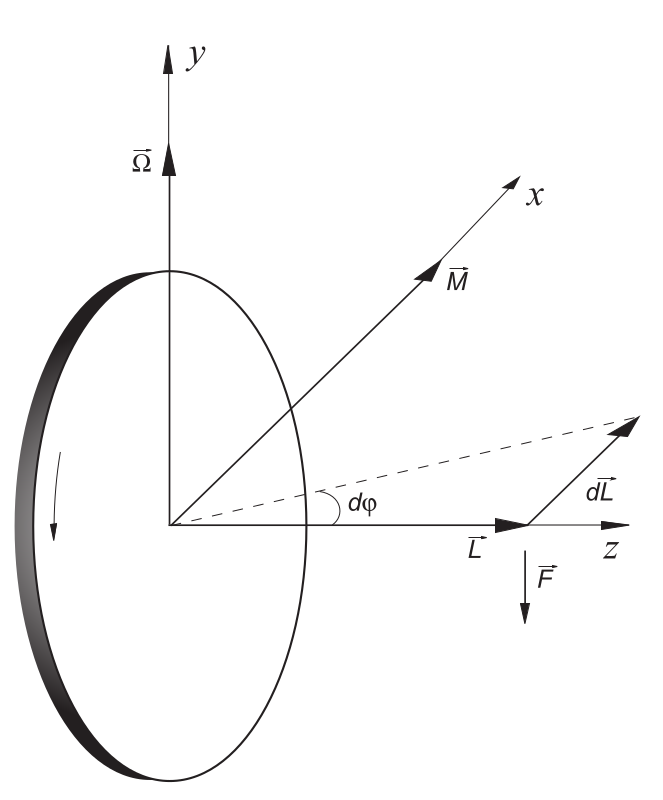
\includegraphics[scale=0.3]{./125/рис 1.png} \label{pic:1} \caption[Рис. 1]{Маховик} \end{figure}

Пусть осьвращения повернулась в плоскости по направлению $zx$ на бесконечно малый угол $d\varphi$. Такой поворот означает добавочное вращение маховика вокруг оси $y$, так что \[d\varphi = \Omega dt\], где $\Omega$ - угловая скорость такого вращения. будем предполагать, что
\begin {equation} L_\Omega \ll L_{\omega_0} \label{eq:5} \end {equation}

\[ dL = L d\varphi = L \Omega dt \]
\[ d\vec{L} = \vec{\Omega} \times \vec{L} dt \]
\begin{equation} \frac{d\vec{L}}{dt} = \vec{\Omega} \times \vec{L} \label{eq:6} \end{equation}
\begin{equation} \vec{M} = \vec{\Omega} \times \vec{L} \label{eq:7} \end{equation}

Вращение гироскопа с угловой скоростью $\Omega$ называется регулярной прецессией гироскопа.

Для гироскопа массой $\m{г}$, у которого ось собственного вращения наклонена на угол $\alpha$ от вертикали, скорость прецессии, происходящей под действием силы тяжести равна
\begin{equation} \Omega = \frac{M}{I_z \omega_0 \sin{\alpha}} = \frac{\m{г} g \l{ц} \sin{\alpha}}{I_z \omega_0 \sin{\alpha}} = \frac{\m{г} g \l{ц}}{I_z \omega_0} \label{eq:8} \end{equation}
где $\l{ц}$ — расстояние от точки подвеса до центра масс гироскопа.

Для изучения регулярной прецессии уравновешенного гироскопа к его оси подвешивают дополнительные грузы. В таком случае скорость прецессии равна
\begin{equation} \Omega = \frac{mgl}{I_z \omega_0} \label{eq:9} \end{equation}
где $m$ - масса груза, $l$ - расстояние от центра карданова подвеса до точки крепления груза \ref{pic:3}.

В данной работе исследуется регулярная прецессия уравновешенного гироскопа.

\begin{figure} [h]
  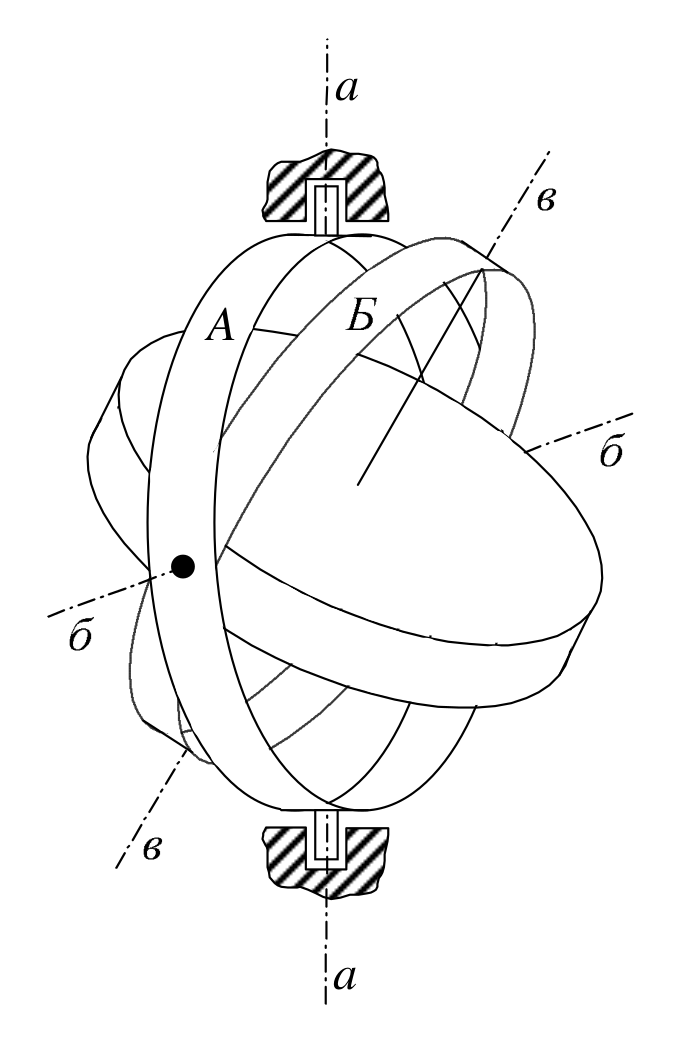
\includegraphics[scale=0.3]{./125/рис 2.png} \label{pic:2}
  \caption[Рис. 2]{Гироскоп в кардановом подвесе}
  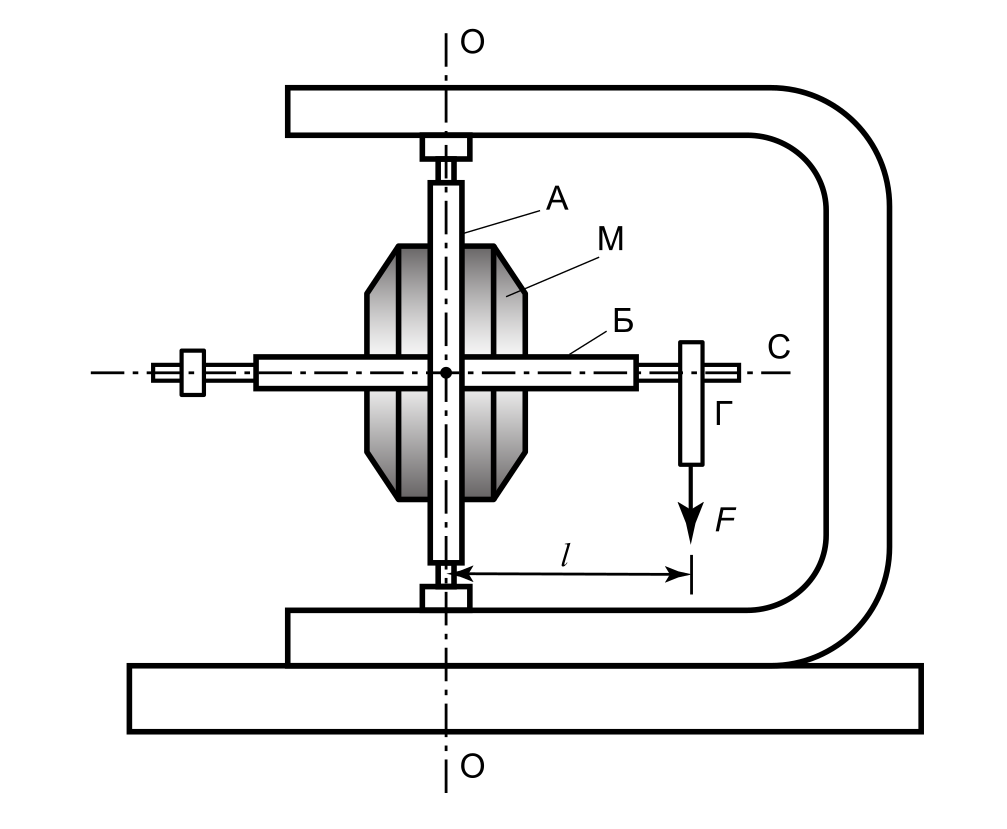
\includegraphics[scale=0.3]{./125/рис 3.png} \label{pic:3}
  \caption[Рис. 3]{Схема экспериментальной установки}
\end{figure}

\begin{equation} T_0 = 2\pi\frac{I_0}{f} \label{eq:10} \end{equation}
где $T_0$ - период крутильных колебаний, $f$ - модуль кручения проволки.
\begin{equation} I_0 = I_{\text{ц}} \frac{T_0^2}{T_{\text{ц}}^2} \label{eq:11} \end{equation}
где $I_\text{ц}$ - момент инерции цилиндра, $T_\text{ц}$ - период крутильных колебаний цилиндра.

\section{Выполнение.}
\begin{enumerate}
  \item \label{Выполнение:1} Установим осъ гироскопа в горизонтальное положение, осторожно поворачивая ее за рычаг С.
  \item \label{Выполнение:2} Включим питание гироскопа и подождем 4-5 мин‚ чтобы вращение ротора успело стабилизироваться.
  \item \label{Выполнение:3} Убедимся в том, что ротор вращается достаточно быстро: при легком постукивании по рычагу С гироскоп не должен изменять своего положения. Поиграемся с гироскопом.
  \item \label{Выполнение:4} Подвесим к рычагу С груз. При этом должна начаться прецессия гироскопа. Трение в оси приводит к тому, что рычаг С начинает медленно опускаться.
  \item \label{Выполнение:5} Отклоним рычаг С на 5-6 градусов вверх от горизонтальной плоскости. Подвесим к нему груз и с помощью секундомера найдем угловую скорость регулярной прецессии по числу оборотов и времени прецессии. Измерения будем продолжать до тех пор, пока рычаг С не опустится на 5-6 градусов ниже горизонтальной плоскости, сделав целое число оборотов. Измерьте также скорость опускания рычага С. Повторим этот опыт не менее пяти раз (хотя бы 2 раза, если значения не совпадут, проделайте 5 раз). Усредним полученные результаты.
  \item \label{Выполнение:6} Проделаем всю серию экспериментов, описанных B пункте 5 при 5-7 значениях момента М силы F относительно центра масс гироскопа. (длина плеча l указана на установке) (см. таблицу (\ref{table:3})). Результаты опытов изобразим в виде графика $\Omega$ в зависимости от М. См. рисунок (\ref{pic:4}). \\
  
В данной таблице $\sigma$ и $\varepsilon$ - абс. и отн. погрешности величин; m - масса груза, подвешенного на расстоянии $\ell$ от гироскопа; n - кол-во оборотов гироскопа; T - период прецессии (т.к. время измерялось секундомером, $\sigma_{T} = \frac{0,6\ \sec}{nT}$); $\Omega$ - угловая скорость прецессии; M - момент сил гироскопа; $\omega_0$ и $\nu_0$ - угловая скорость и частота вращения ротора гироскопа.

Так как массы грузов и длина $\ell$ была измерена до нас, будем считать, что их погрешность определяется последним знаком, т.е.

\begin{table} [h] \center
\begin{tabular}{l|l|l|l}
&значение&$\sigma$&$\eps$\\
\hline
$\ell$, см&12,1&0,1&0,8\%\\
g, м/$\sec^2$&9,81523&0,00001&$10^{-4}$\%\\
время, с&&0,6&\\
масса, г&&1&\\
\end{tabular}
\caption[Таблица 1]{Характерные величины \label{table:1}}
\end{table}


% таблица 1
\begin{table} [h]
\resizebox {\textwidth} {!} {
\begin{tabular} {l|llllllllll}
измерение&1&2&3&4&5&6&7&8&9&10\\
\hline
m, г&329&329&217&217&142&142&91&91&57&57\\
n&23&21&10&10&10&10&5&5&5&5\\
T, с&31.12&31.23&47.10&47.04&72.06&71.82&111.96&112.08&182.16&181.85\\
$\sigma_{T}$, с&0.03&0.03&0.06&0.06&0.06&0.06&0.12&0.12&0.12&0.12\\
$\eps_{T}$&0.08\%&0.09\%&0.13\%&0.13\%&0.08\%&0.08\%&0.11\%&0.11\%&0.07\%&0.07\%\\
$\Omega$, рад/c&0.20189&0.20120&0.13340&0.13357&0.08719&0.08749&0.05612&0.05606&0.03449&0.03455\\
$\sigma_{\Omega}$, рад/с&0.00017&0.00018&0.00017&0.00017&0.00007&0.00007&0.00006&0.00006&0.00002&0.00002\\
$\eps_{\Omega}$&0.08\%&0.09\%&0.13\%&0.13\%&0.08\%&0.08\%&0.11\%&0.11\%&0.07\%&0.07\%\\
M, Н*м&0.390&0.390&0.258&0.258&0.169&0.169&0.108&0.108&0.067&0.067\\
$\sigma_{M}$, Н*м&0.003&0.003&0.002&0.002&0.002&0.002&0.001&0.001&0.001&0.001\\
$\eps_{M}$&0.88\%&0.88\%&0.95\%&0.95\%&1.09\%&1.09\%&1.37\%&1.37\%&1.95\%&1.95\%\\
$\w_0$, рад/c&2515&2524&2519&2516&2516&2507&2509&2512&2541&2537\\
$\nu_0$, Гц&400&402&401&400&400&399&399&400&404&404\\
\end{tabular} 
}
\caption{Измерения \label{table:2}}
\end{table}


\begin{table} [h] \center
\begin{tabular}{l|l|l|l|l}
m, г&n&T, с&$\Omega$, рад/с&M, Н*м\\
\hline
 329 &22& 31 & 0,2 & 0,39 \\
 217 &10& 47 & 0,13 & 0,26 \\
 142 &10& 72 & 0,09 & 0,17 \\
 91 &5& 112 & 0,06 & 0,11 \\
 57 &5& 182 & 0,03 & 0,07 \\
\end{tabular}
\caption{Упрощенная таблица \ref{table:2} \label{table:3}}
\end{table}

\begin{figure} [h] \center
	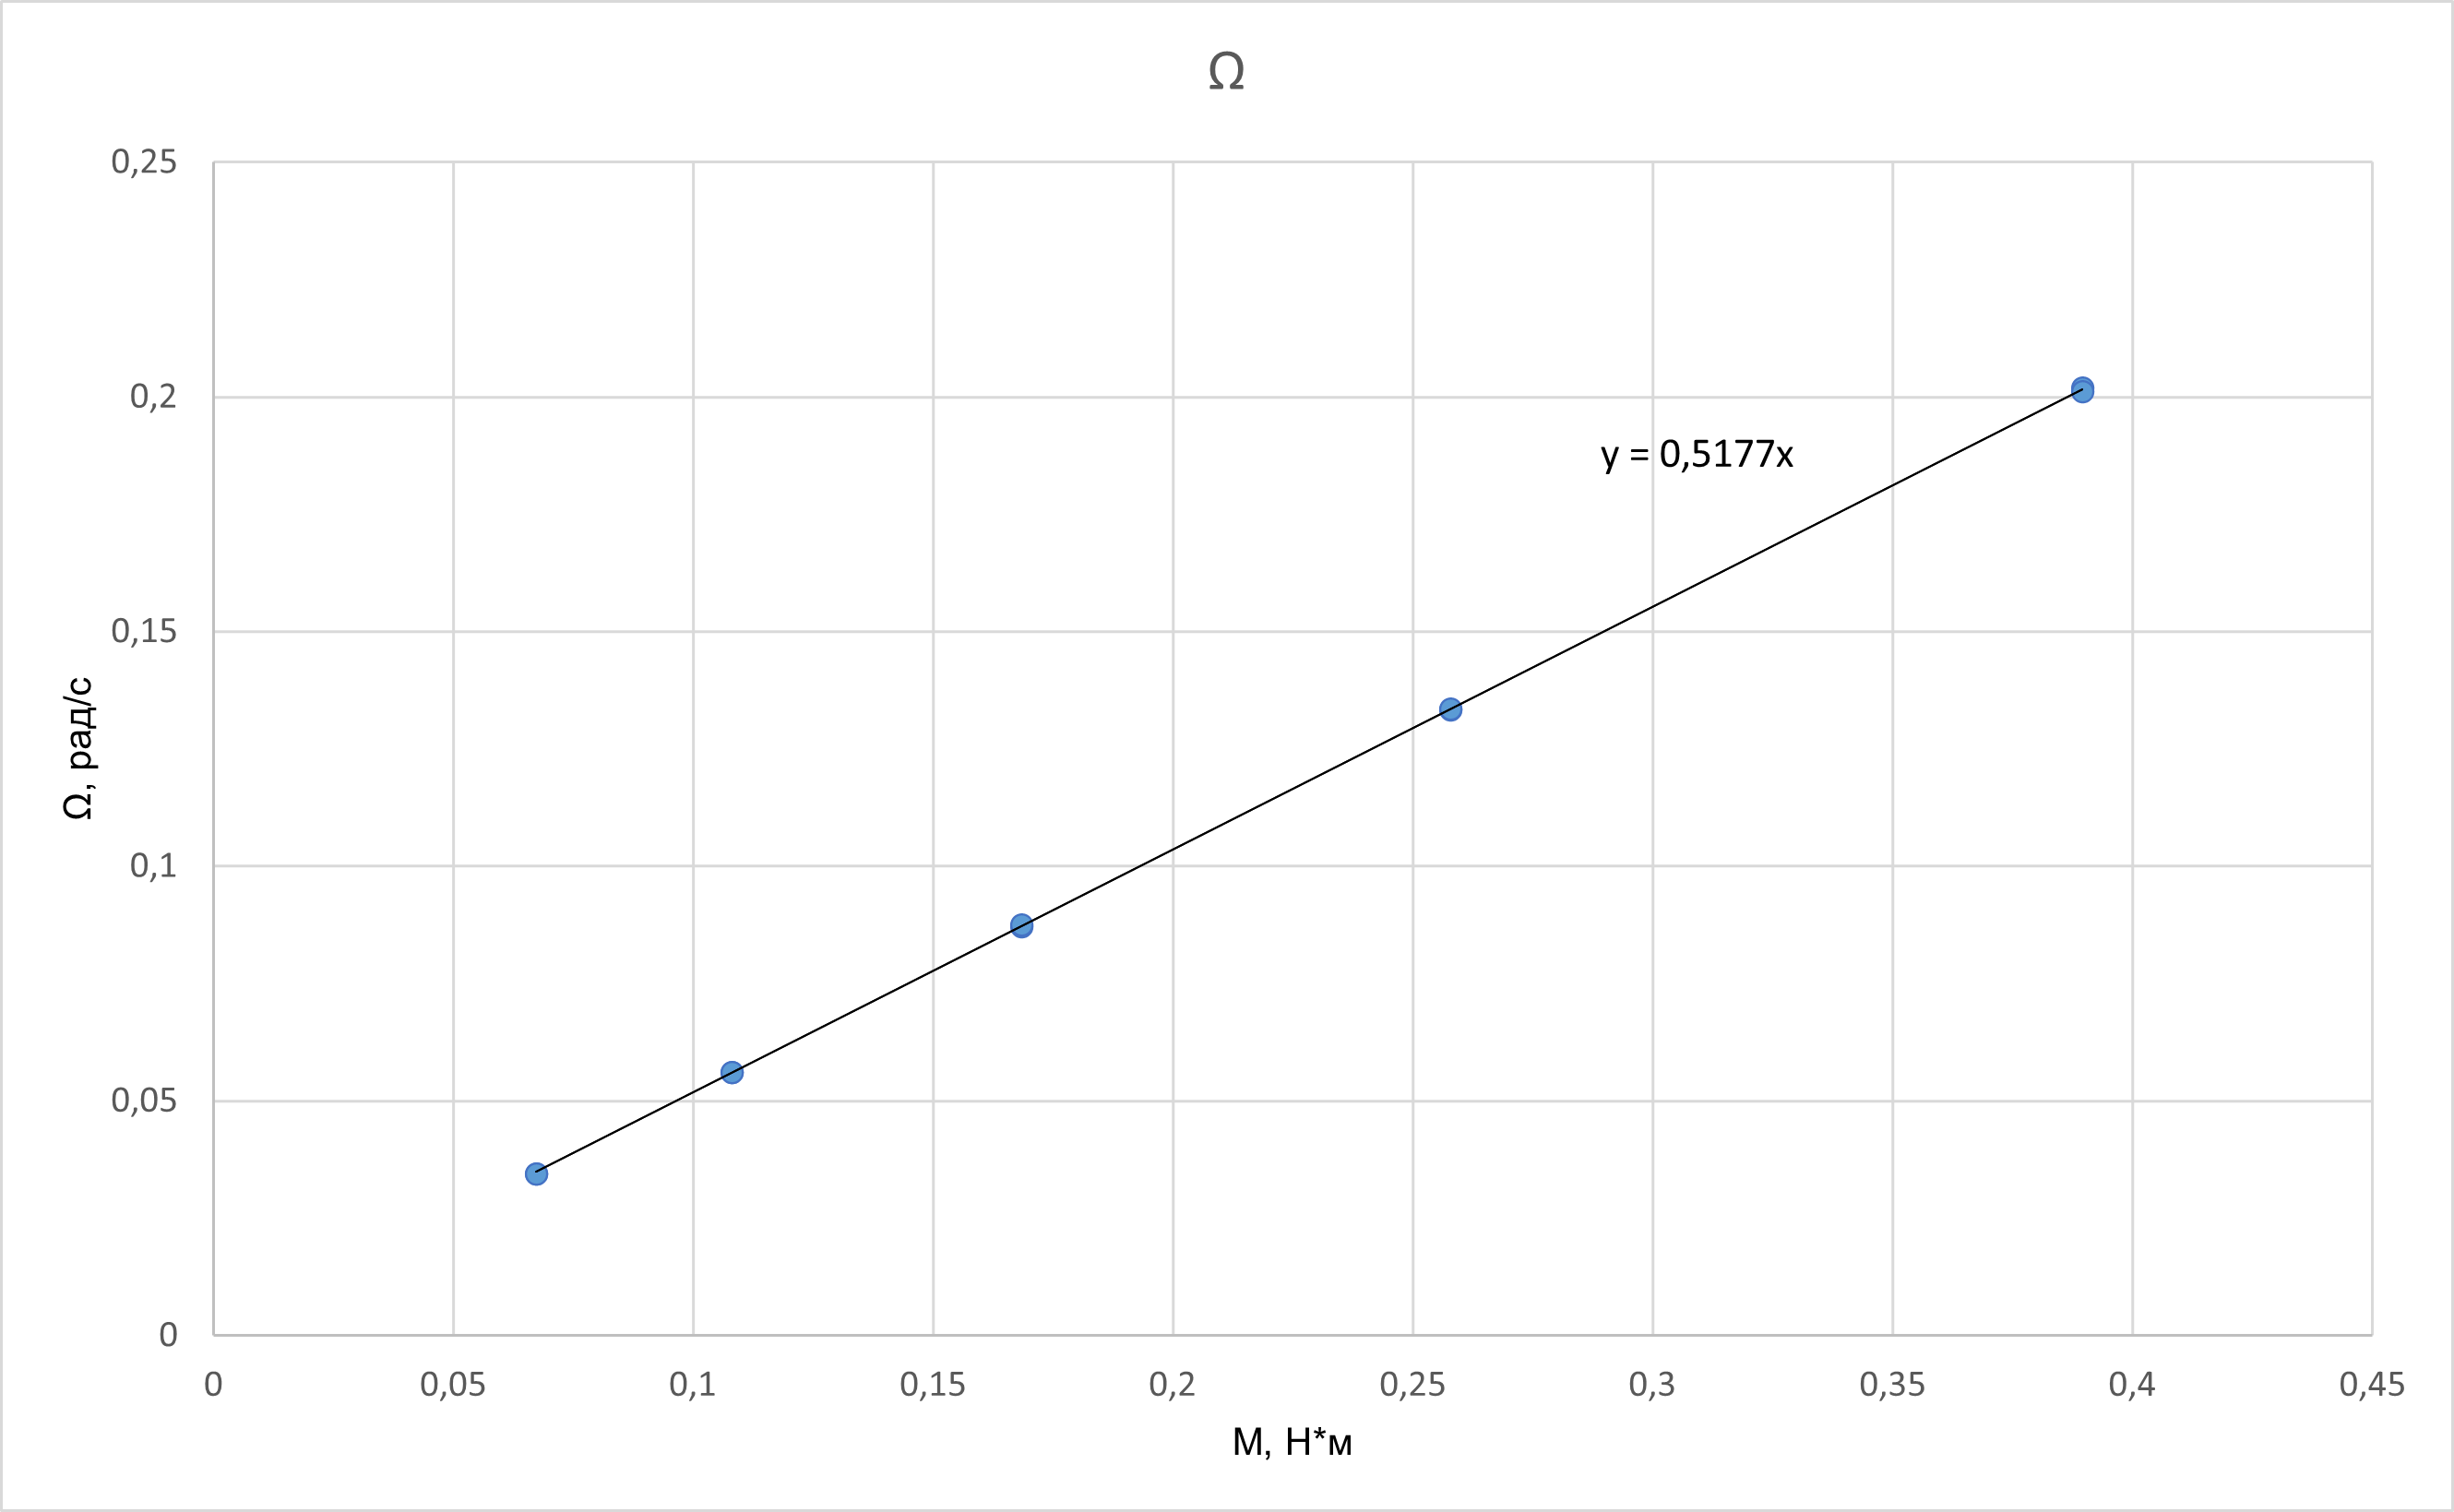
\includegraphics[scale=0.8]{./125/graph1.png}
	\label{graph:1} \label{pic:4}
	\caption[Рис. 4]{График зависимости $\Omega$ (скорости прецессии) от М (момента сил)}
\end{figure}

По наклону прямой можно найти моиент импульса: 
$L = (1,93 \pm 0,03) \frac{\text{кг}\ \text{м}^2}{\text{с}}$

\newpage

  \item \label{Выполнение:7} Измерим момент инерции ротора гироскопа относительно оси симметрии. Для этого подвесим ротор, извлеченный из такого же гироскопа, к концу вертикально висящей проволоки так, чтобы ось симметрии гироскопа была вертикальна, и измерим период крутильных колебаний получившегося маятника. Заменим ротор гироскопа цилиндром, для которого известны или легко могут быть измерены радиус и масса, и определим для него период крутильных колебаний. Пользуясь формулой \eqref{eq:11}, вычислим момент инерции ротора гироскопа.
  % таблица 2
\begin{table} [h] \center
\begin{tabular}{l|lll}
&Значение&$\sigma$&$\varepsilon$\\
\hline
m, г&1617&1&0,1\%\\
D, см&7,80&0,01&0,1\%\\
R, см&3,900&0,005&0,1\%\\
$I_\text{ц}$&0,001229&$3\cdot10^{-6}$&0,3\%\\
$T_1$&80,2&0,6&0,7\%\\
$T_2$&80,3&0,6&0,7\%\\
$T_\text{ц}$&80,28&0,6&0,7\%\\
\hline
$T_1$&63,4&0,6&1\%\\
$T_2$&63,5&0,6&1\%\\
$T_0$&63,4&0,6&1\%\\
\end{tabular}
\caption{Характеристики цилиндра \label{table:4}}
\end{table}

\[ I_0 = 0,77\ \text{г}\cdot\text{м}^2 \]

  \item \label{Выполнение:8} Оценим погрешности в определении $\Omega$ и $I_0$:

$\sigma_{I_0} = 0,01\ \text{г}\cdot\text{м}^2$
$\varepsilon_{I_0} = 2\%$

\[ I_0 = (0,77 \pm 0,01)\ \text{г}\cdot\text{м}^2 \]

$\sigma_{\Omega} = \Omega \cdot \varepsilon_{\Omega} = \frac{2\pi}{T^2} \sigma_{T}$ ; $\varepsilon_{\Omega} = \varepsilon_T$ См. таблицу \ref{table:2}.

  \item \label{Выполнение:9} Рассчитайте с помощью \eqref{eq:9} частоту вращения ротора гироскопа.

$\eqref{eq:9} \implies \omega_0 = \frac{M}{\Omega I_0},\ 
\nu_0 = \frac{\omega_0}{2\pi}$
См. таблицу \ref{table:2} и \ref{table:5} \\
\[ \average{\omega_0} = 2516\ \frac{\text{рад}}{\text{с}},\ 
\average{\nu_0} = 400\ \text{Гц} \]

Также найдем погрешности $\w_0$ и $\nu_0$:
\[ \average{\sigma_{\w_0}} = 45\ \frac{\text{рад}}{\text{с}},\ 
\average{\sigma_{\nu_0}} = 7\ \text{Гц} \]
\[ \average{\varepsilon_{\w_0}} = \average{\varepsilon_{\nu_0}} = 1,7 \% \]
 
В итоге:
\[ \w_0 = (2516 \pm 45)\ \ \frac{\text{рад}}{\text{с}},\ 
\nu_0 = (400 \pm 7)\ \text{Гц} \]

\begin{table} [h] \center
\begin{tabular}{l|l|l|l|l|l}
&Значение&$\sigma^{\text{приб}}$&$\sigma^{\text{случ}}$&$\sigma$&$\varepsilon$\\
\hline
$\w_0$, рад/c&2516&43& 11 & 45 &1,8\%\\
$\nu_0$, Гц&400&7& 2 & 7 &1,8\%\\
\end{tabular}
\caption[Таблица 4]{$\w_0$ и $\nu_0$ \label{table:5}}
\end{table}


  \item \label{Выполнение:10} Пo скорости опускания рычага С во время прецессии определите момент сил трения.

Для определения угла, на который опуститься гироскоп, нужно использовать транспортир в виде треугольника. Мы не догадались использовать транспортир и опирались только на разметку на гироскопе. Взгляните на таблицу \ref{table:2}, первое измерение было сделано при 23 полных оборотах, второе - при 10, последнее - при 5. Учитывая, что маятник опускался очнь медленно, и мы бы не успели проделать все измерения корректно. Момент сил трения в оси гироскопа можно найти по формуле \eqref{eq:7}:

$\vec{M_\text{тр}}= \vec{\omega} \times \vec{L}$, где $\omega$ - угловая скорость опускания гироскопа, $\vec{L}$ - момент импульса гироскопа. $\vec{L} = I_0 \vec{\w_0}$, $I_0$ и $\w_0$ мы находили в пункте \ref{Выполнение:7} и \ref{Выполнение:9}.

$M_\text{тр} = \frac{\varphi}{n T} \cdot I_0 \w_0 = \frac{\pi \theta}{180 n T} \cdot I_0 \w_0$, где $\theta$ - угол поворота в градусах, n - кол-во оборотов, T - период.
Если считать, что в первом измерении гироскоп опустился на 5 градусов:
\[ M_\text{тр} \thickapprox (0.00024 \pm 0.00005)\ \H \cdot \m \]
$\varepsilon_{M_\text{тр}} \thickapprox 20\%$

  \item \label{Выполнение:11} Определите частоту вращения ротора гироскопа пo фигурам Лиссажу.
  
  Для этого включим осциллограф и генератор. Переключателем «Множитель частоты» и ручкой «Hz» на генераторе добьемся того, что-бы на экране осциллографа появилась фигура, похожая наэллипс. Подберите частоту генератора так, чтобы эллипс стал неподвижным. Если этого сделать не удается, то выключите на короткое время питание электромотора гироскопа, чтобы ток первой обмотки не наводил ЭДС во второй и не мешал измерениям. Делать измерения при этомнадо быстро, так как при выключенном питании ротор гироскопа начинает замедлять свое вращение. Получение на экране осциллографа неподвижного эллипса означает, что частота сигнала генератора равна частоте вращения ротора гироскопа.

  У нас получилось, что частота вращения гироскопа примерно равна 400 Гц, что совпадает с измеренной.

  \item \label{Выполнение:12}  Оценим погрешность полученных результатов. Сравним угловые скорости вращения ротора гироскопа, определяемые разными методами.

См. пункты \ref{Выполнение:9}, \ref{Выполнение:11} и таблицу \ref{table:5}.

  \item  Убедимся в применимости соотношения \eqref{eq:5} в данной работе.
  
Момент инерции гироскопа не сильно зависит от оси, т.е. $I_{\w_0} \thickapprox I_\Omega$.
$L_{\w_0} = I_{\w_0} \cdot \w_0,\ L_\Omega = I_\Omega \cdot \Omega$
Так как $\w_0 \gg \Omega$, то $L_{\w_0} \gg L_\Omega$, ч.т.д.

\section{Вывод}
В результате данной лабораторной работы мы исследовали вынужденную прецессию гироскопа, установили зависимость скорости вынужденной прецессии от величины момента сил, действующих на ось гироскопа, определить скорость вращения ротора гироскопа и сравнили ее со скоростью, рассчитанной по скорости прецессии.

\end{enumerate}

\end{document}